\chapter{Wind-driven circulation overview}
\label{chap:winddriven}

As discussed the overturning circulation is rather weak in the global ocean, but is very important for the climate as that is how deep water stores heat and carbon.  However, the major ocean currents (other than tides) are typically driven by the winds.  

This chapter provides some data with minimal discussion that shows two example flows that we are interested in for the following chapters.  The first is wind blowing along a coast.  Such a wind drives coastal upwelling and downwelling and is very important for the ecosystem of the coast.   The second is the large-scale circulation of the North Pacific basin.  

\section{Coastal upwelling}

\begin{figure}[hbt]
  \begin{center}
  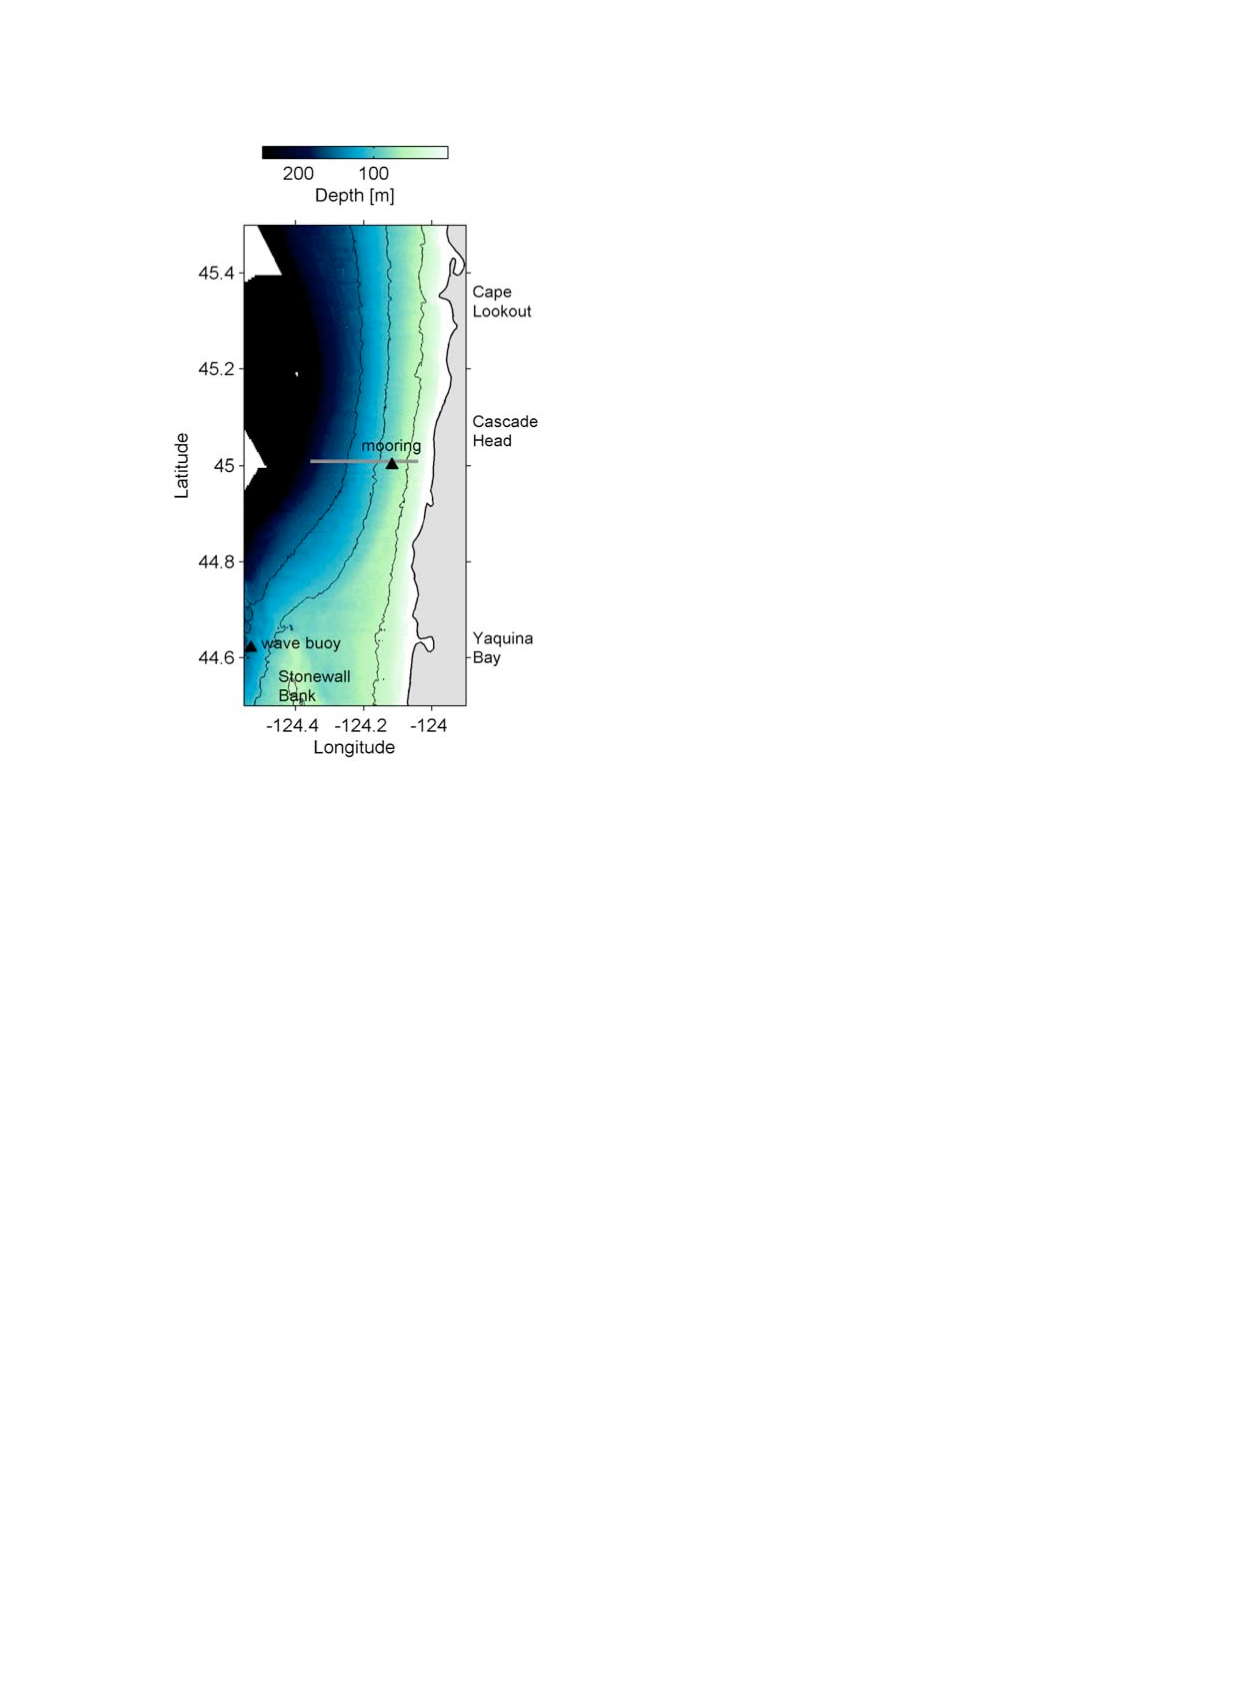
\includegraphics[width=2.5in]{figs/WindOverview/PerlinFig1}
    \caption{Location of coastal observations.  A ship transited the line at 45 N repeatedly over an 8-day period.  }
    \label{fig:PerlinFig1}  
  \end{center}
\end{figure}


\begin{figure}[hbt]
  \begin{center}
  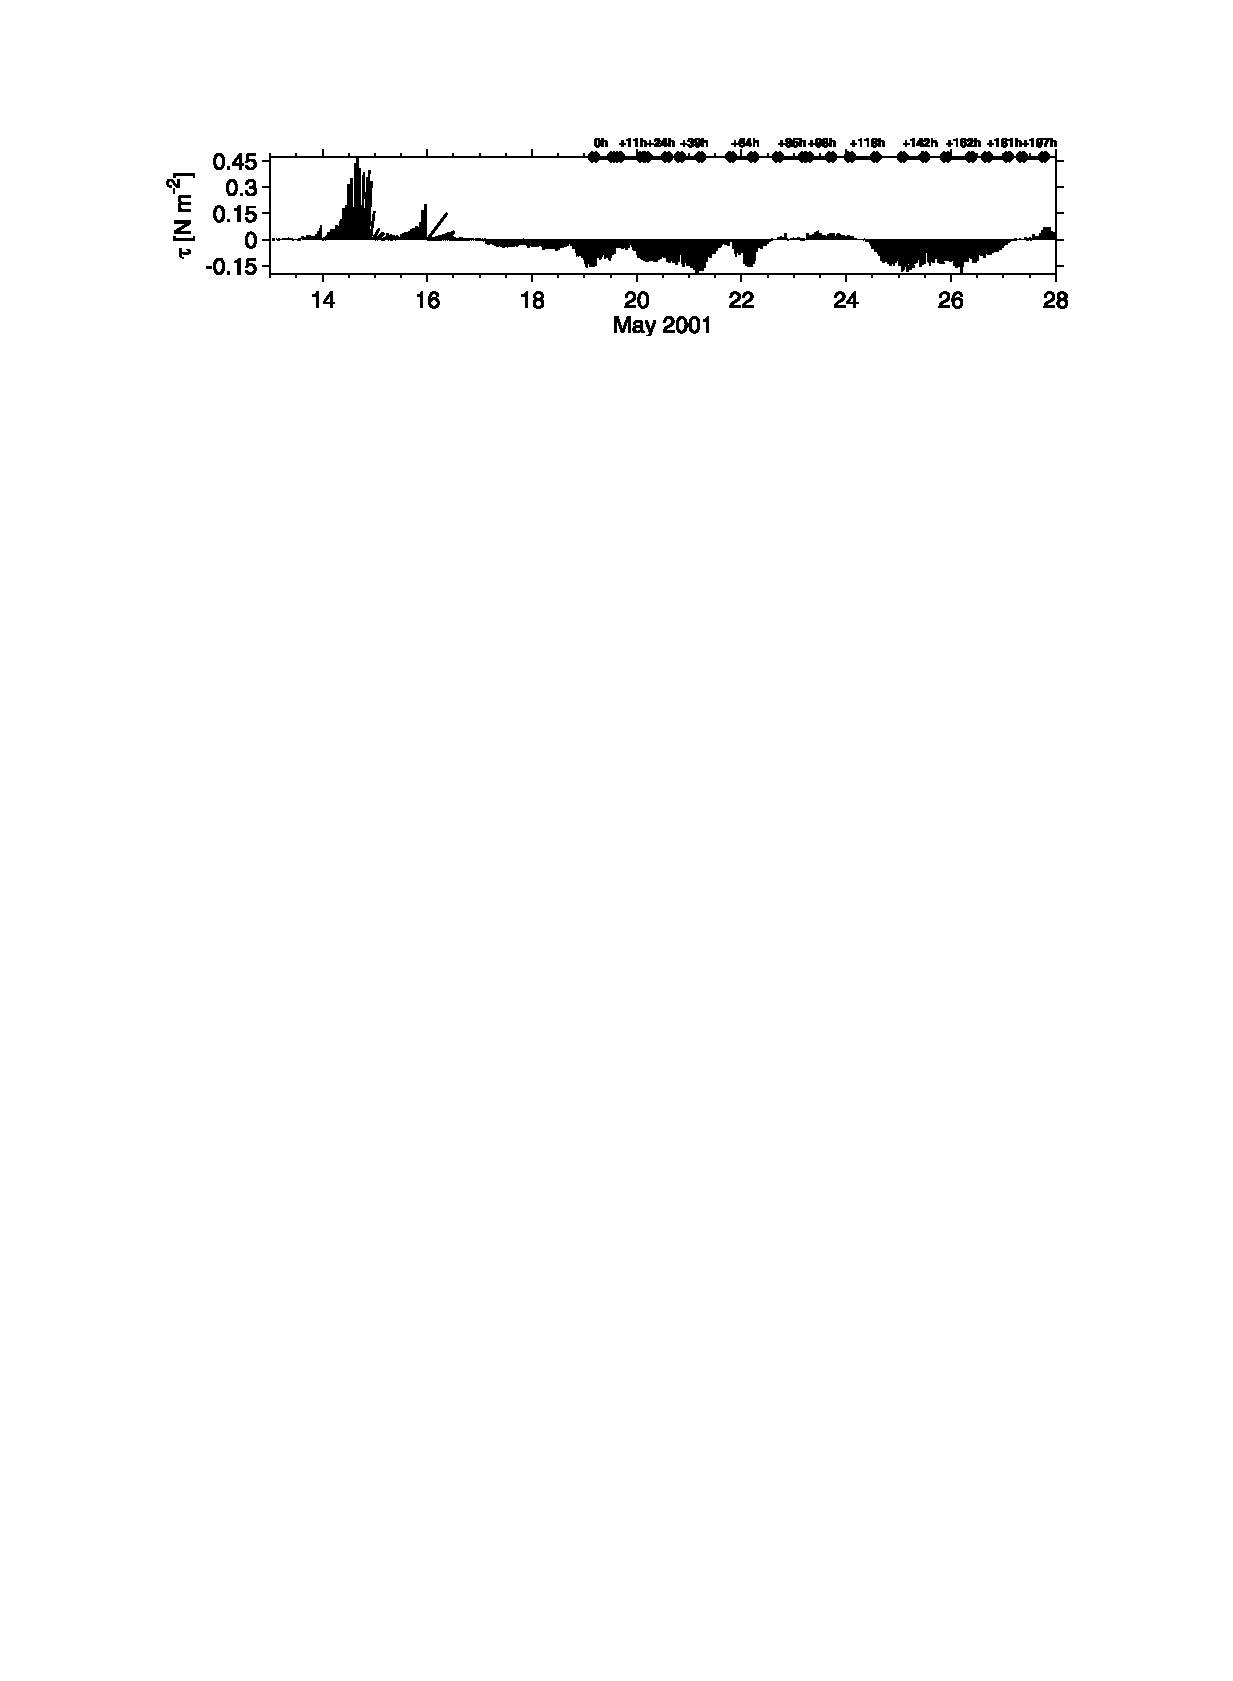
\includegraphics{figs/WindOverview/PerlinFig2}
    \caption{Wind stress arrows, where the wind direction is indicated by the arrow direction, and is mostly north (postive) and south (negative).  During the cruise (dots along top axes, winds were mostly towards the south, except for a brief reversal 23-24 May.  }
    \label{fig:PerlinFig2}  
  \end{center}
\end{figure}

\begin{figure}[hbt]
  \begin{center}
  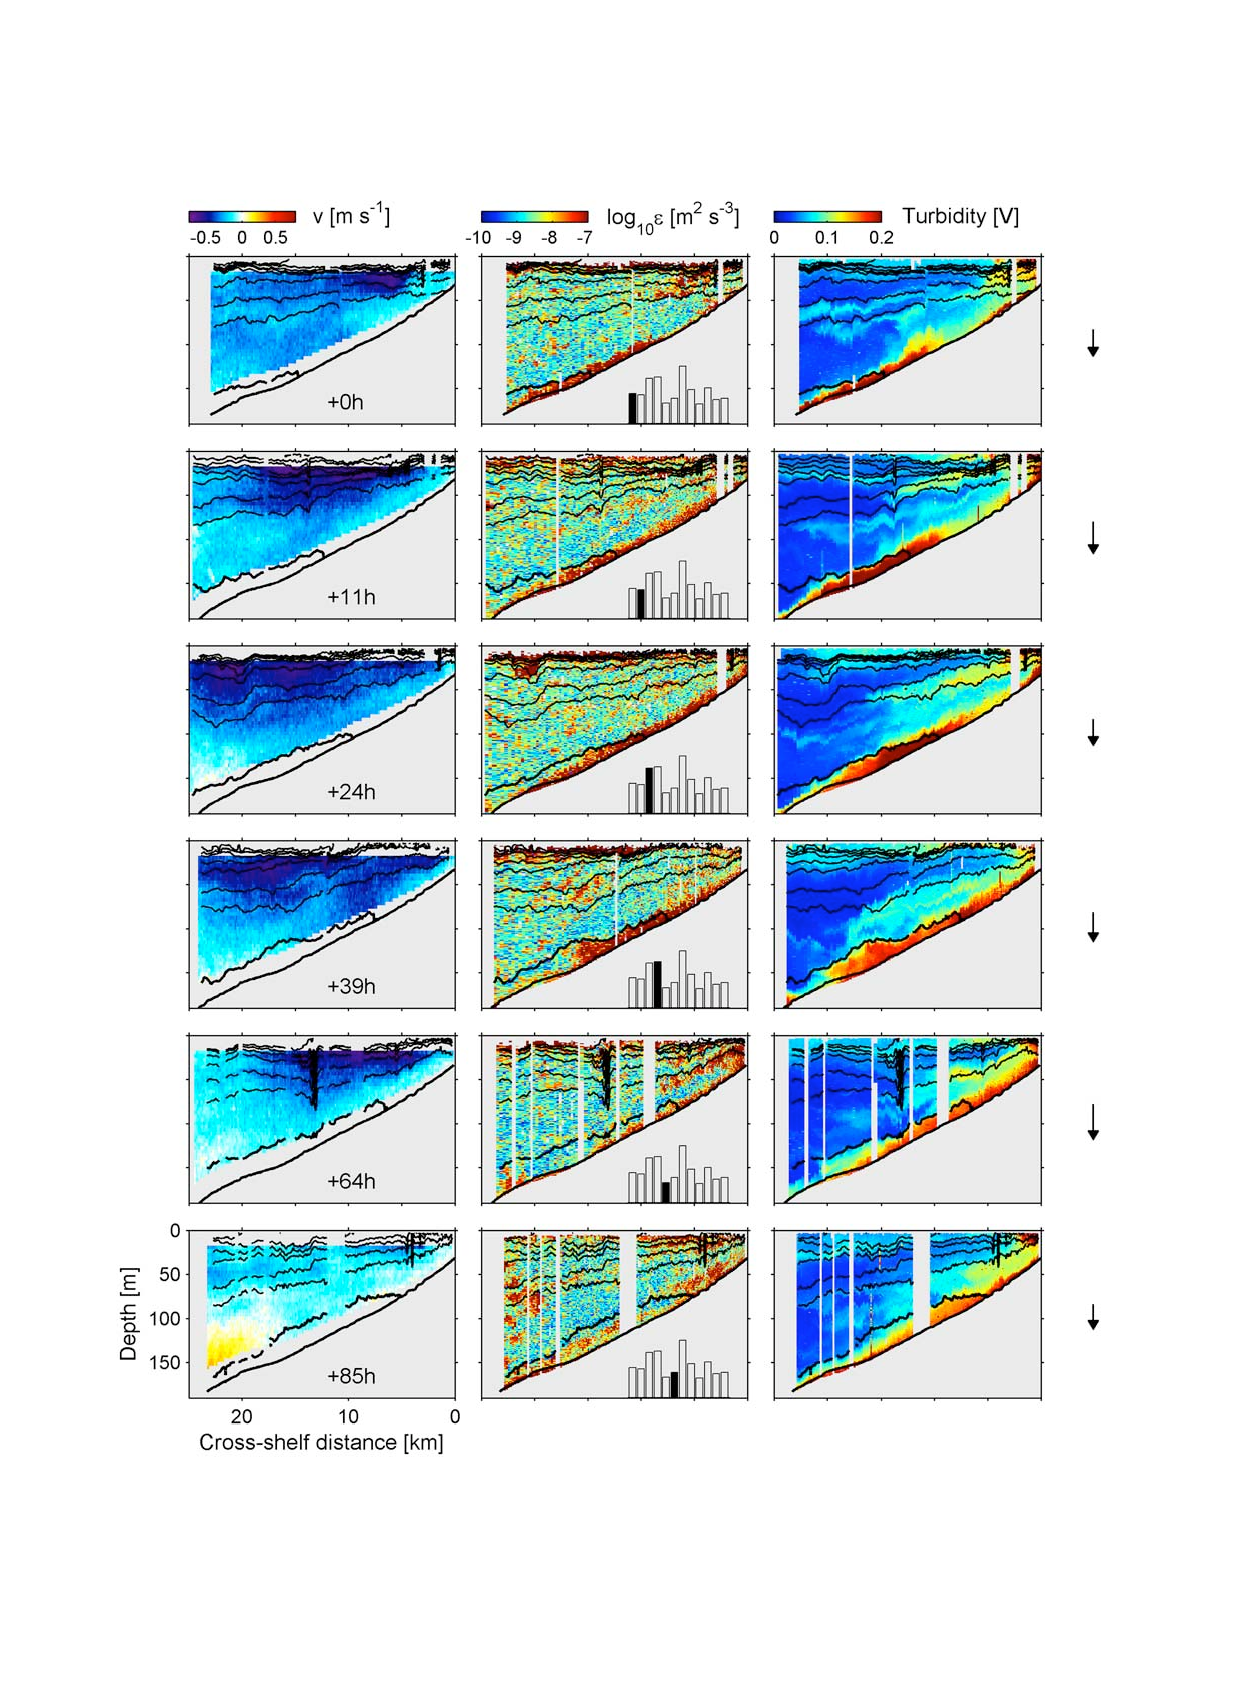
\includegraphics{figs/WindOverview/PerlinFig3a}
    \caption{Observations from the ship.  Black contours are potential density.  The left column shows along-shelf current speed, blue meaning towards the south.  The middle column shows the strength of turbulence in the water column, yellow/red being more turbulent.  The right column shows turbidity, a measure of particles suspended in the water column.  the arrows on the far right are the wind stress vectors.}
    \label{fig:PerlinFig3a}  
  \end{center}
\end{figure}

\begin{figure}[hbt]
  \begin{center}
  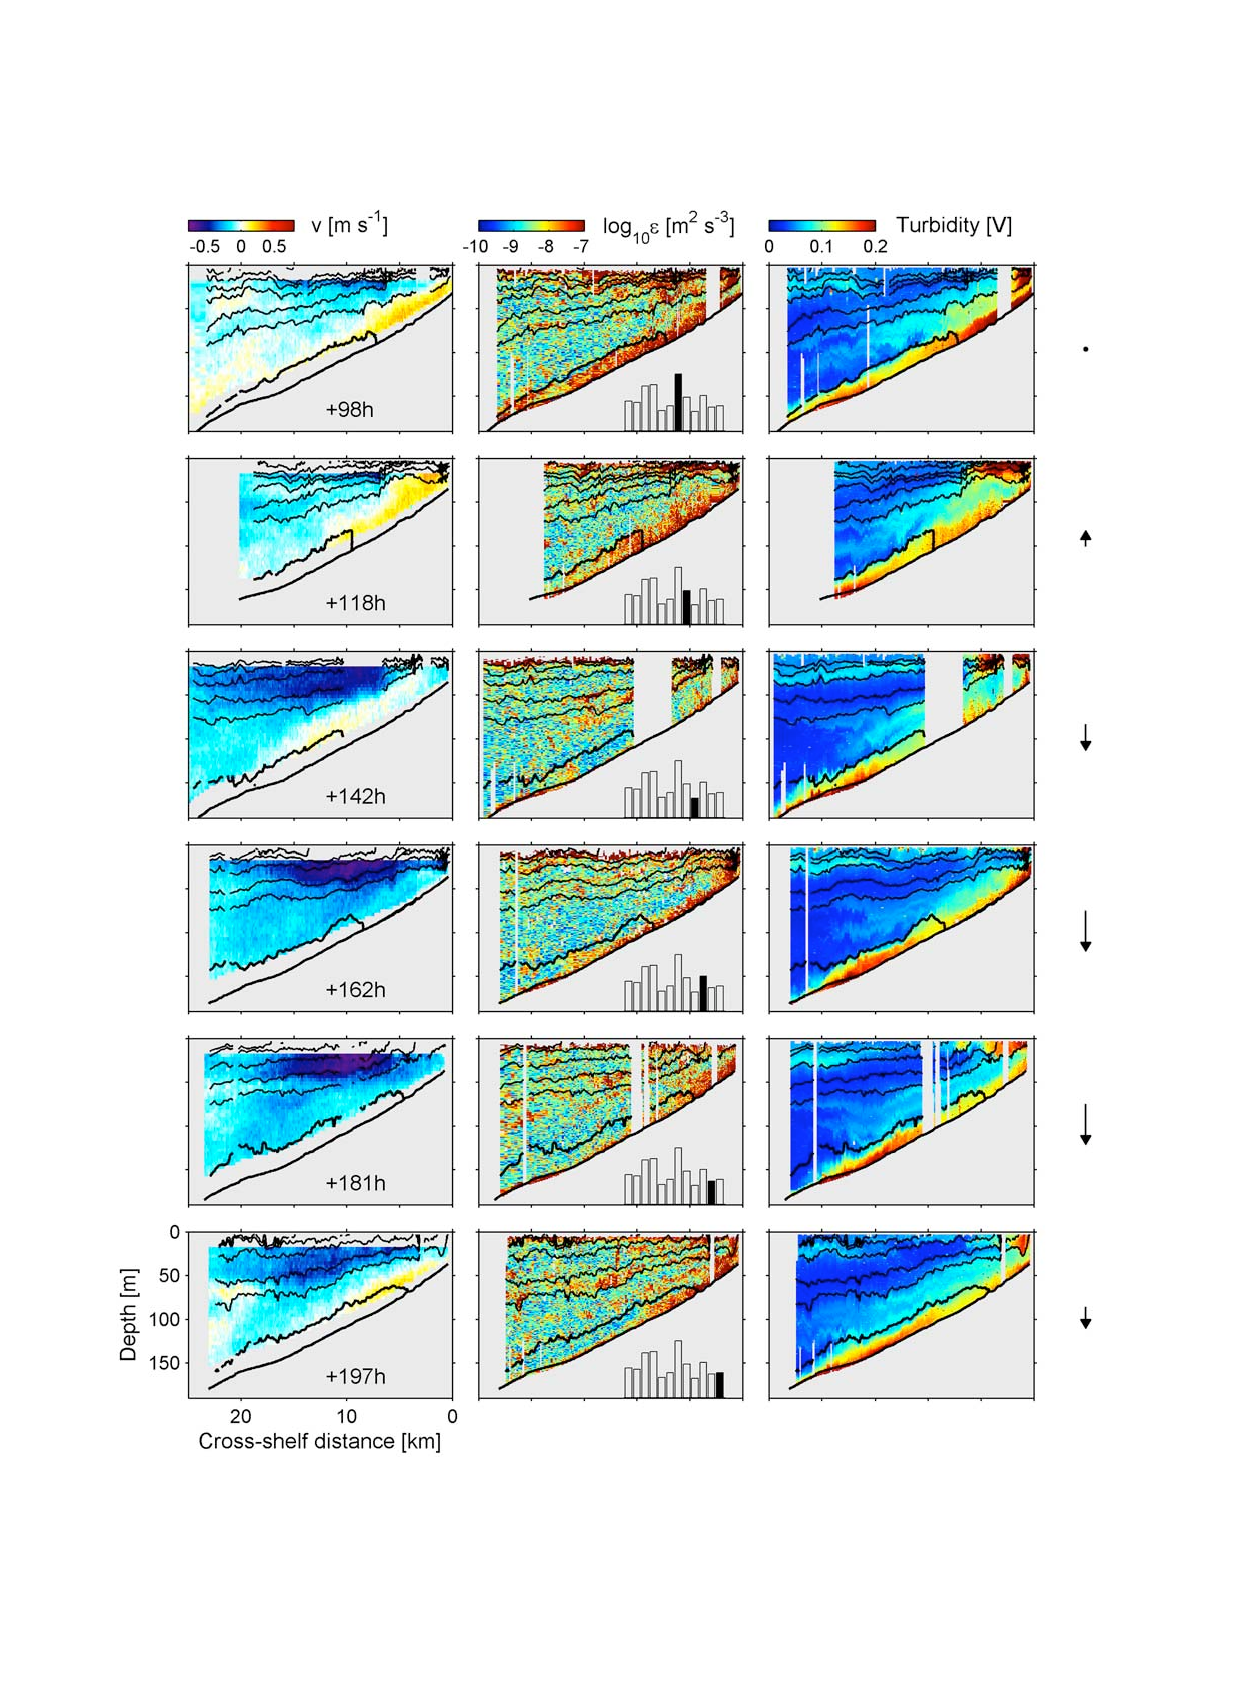
\includegraphics{figs/WindOverview/PerlinFig3b}
    \caption{As in \fref{fig:PerlinFig3a}.  Note the wind reversal and then resumption of wind blowing to the south.}
    \label{fig:PerlinFig3b}  
  \end{center}
\end{figure}

\begin{figure}[hbt]
  \begin{center}
  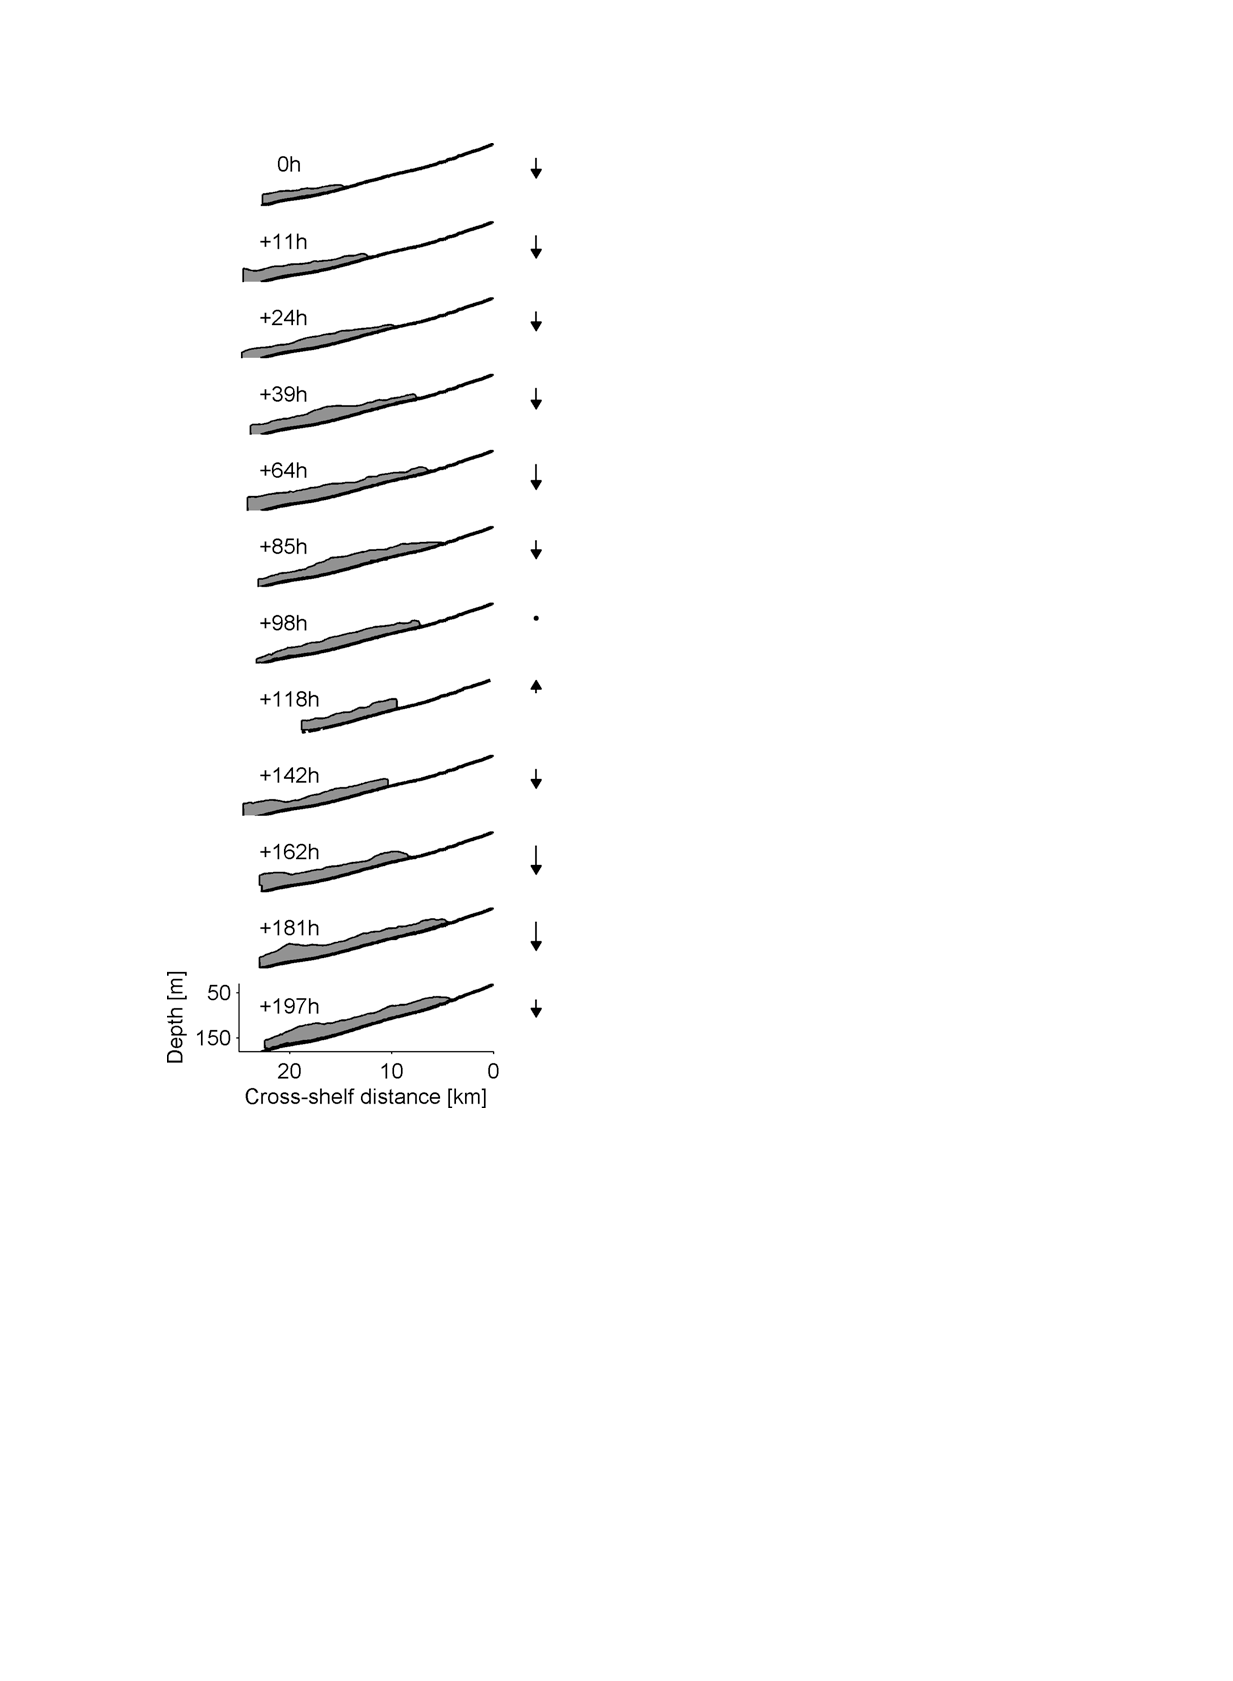
\includegraphics[width=2.7in]{figs/WindOverview/PerlinFig8}
    \caption{Same density data as \fref{fig:PerlinFig3a} and \fref{fig:PerlinFig3b}, highlighting the motion of the bottom boundary layer up and down the shelf.  During peak upwelling the speed is about 6 km/d.}
    \label{fig:}  
  \end{center}
\end{figure}

\clearpage
\section{North Pacific observations} 

\begin{figure}[hbt]
  \begin{center}
  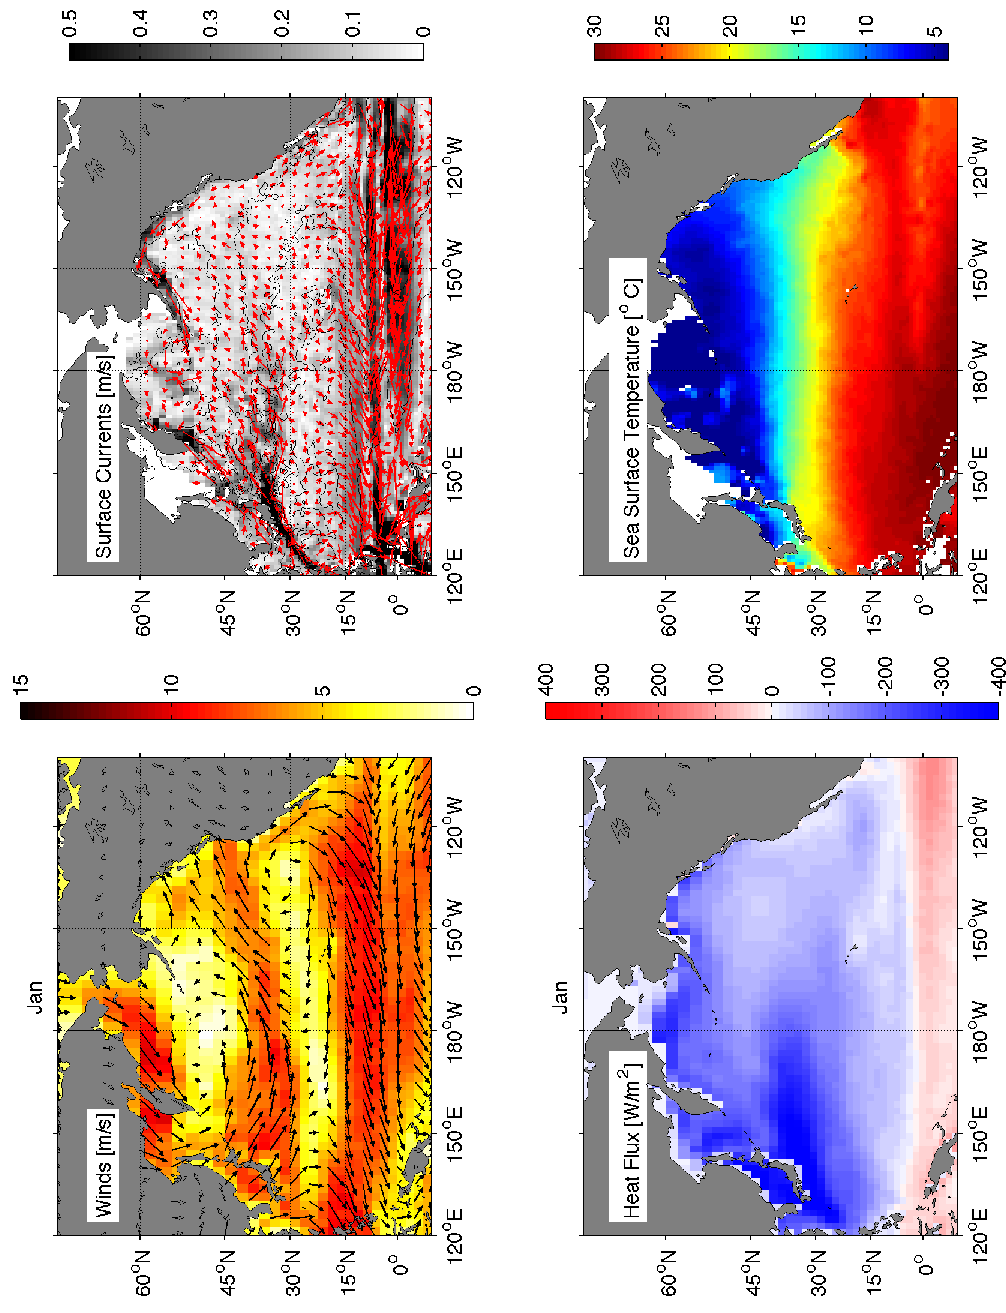
\includegraphics[angle=270]{figs/WindOverview/SurfaceCurrents01}
    \caption{}
    \label{fig:}  
  \end{center}
\end{figure}

\begin{figure}[hbt]
  \begin{center}
  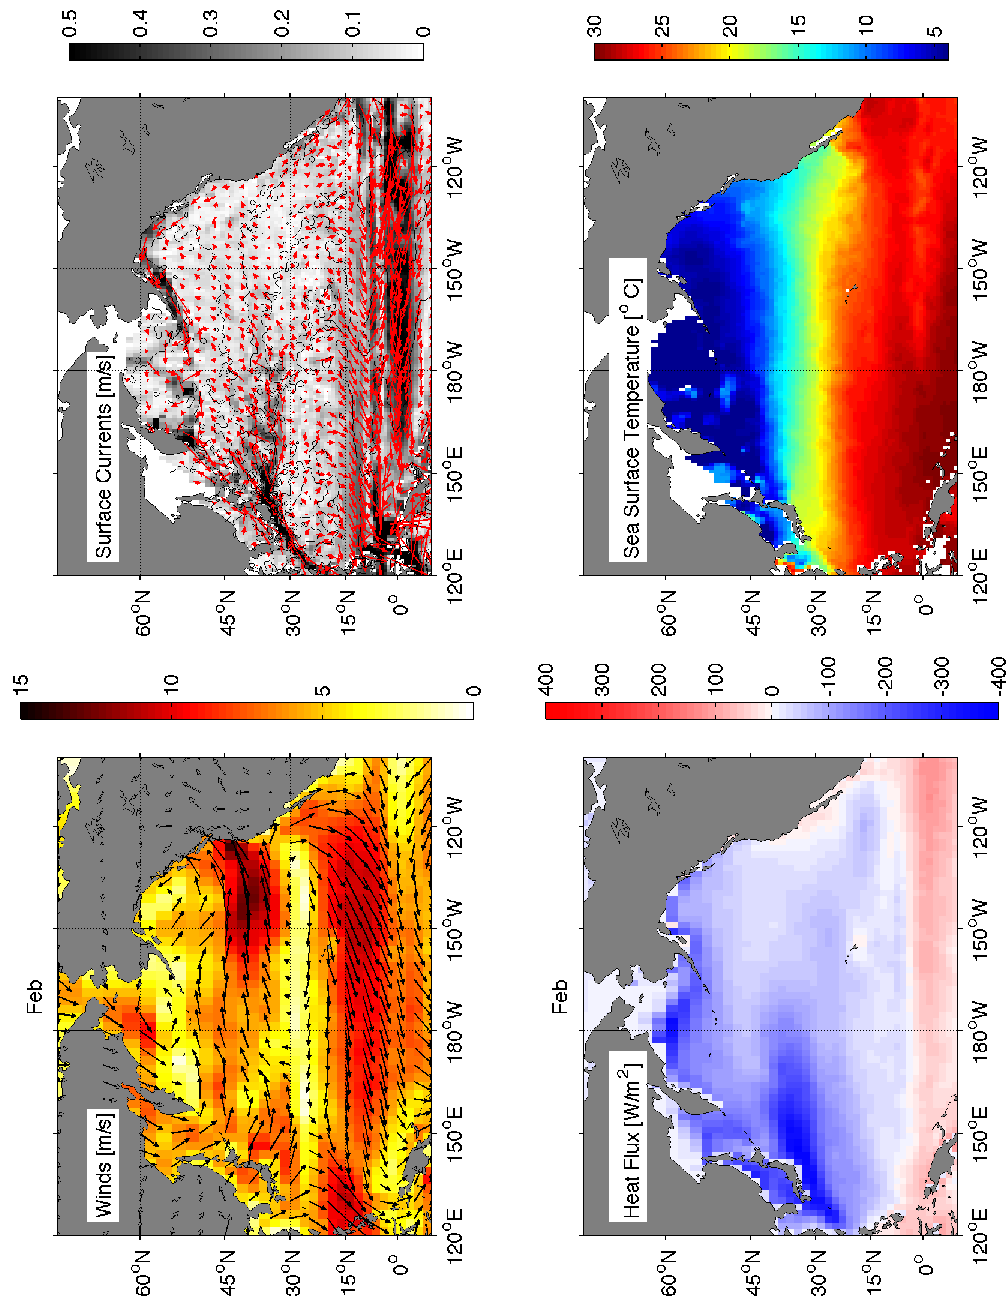
\includegraphics[angle=270]{figs/WindOverview/SurfaceCurrents02}
    \caption{}
    \label{fig:}  
  \end{center}
\end{figure}

\begin{figure}[hbt]
  \begin{center}
  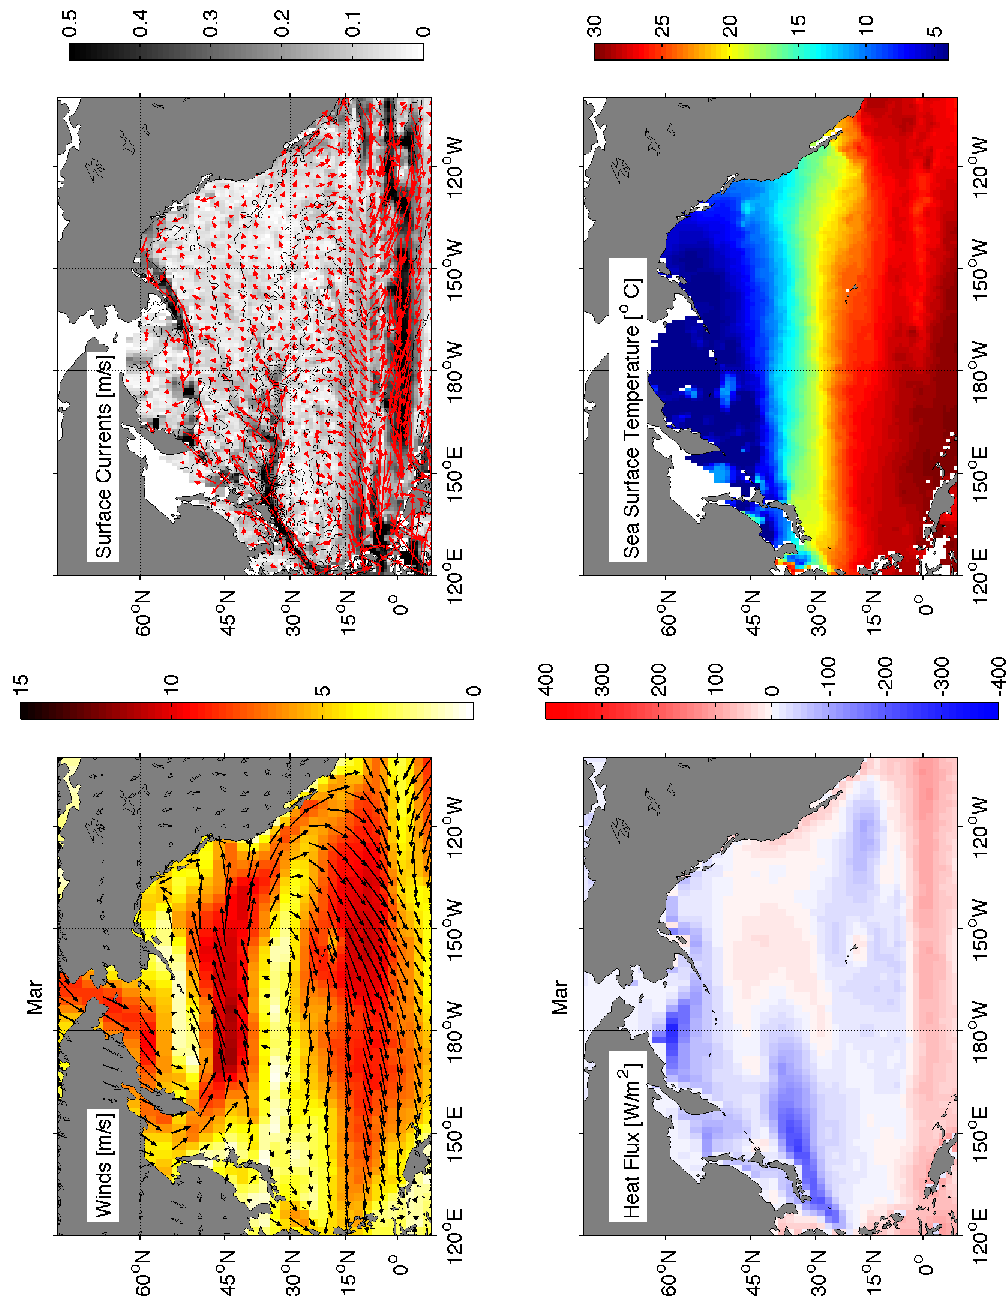
\includegraphics[angle=270]{figs/WindOverview/SurfaceCurrents03}
    \caption{}
    \label{fig:}  
  \end{center}
\end{figure}

\begin{figure}[hbt]
  \begin{center}
  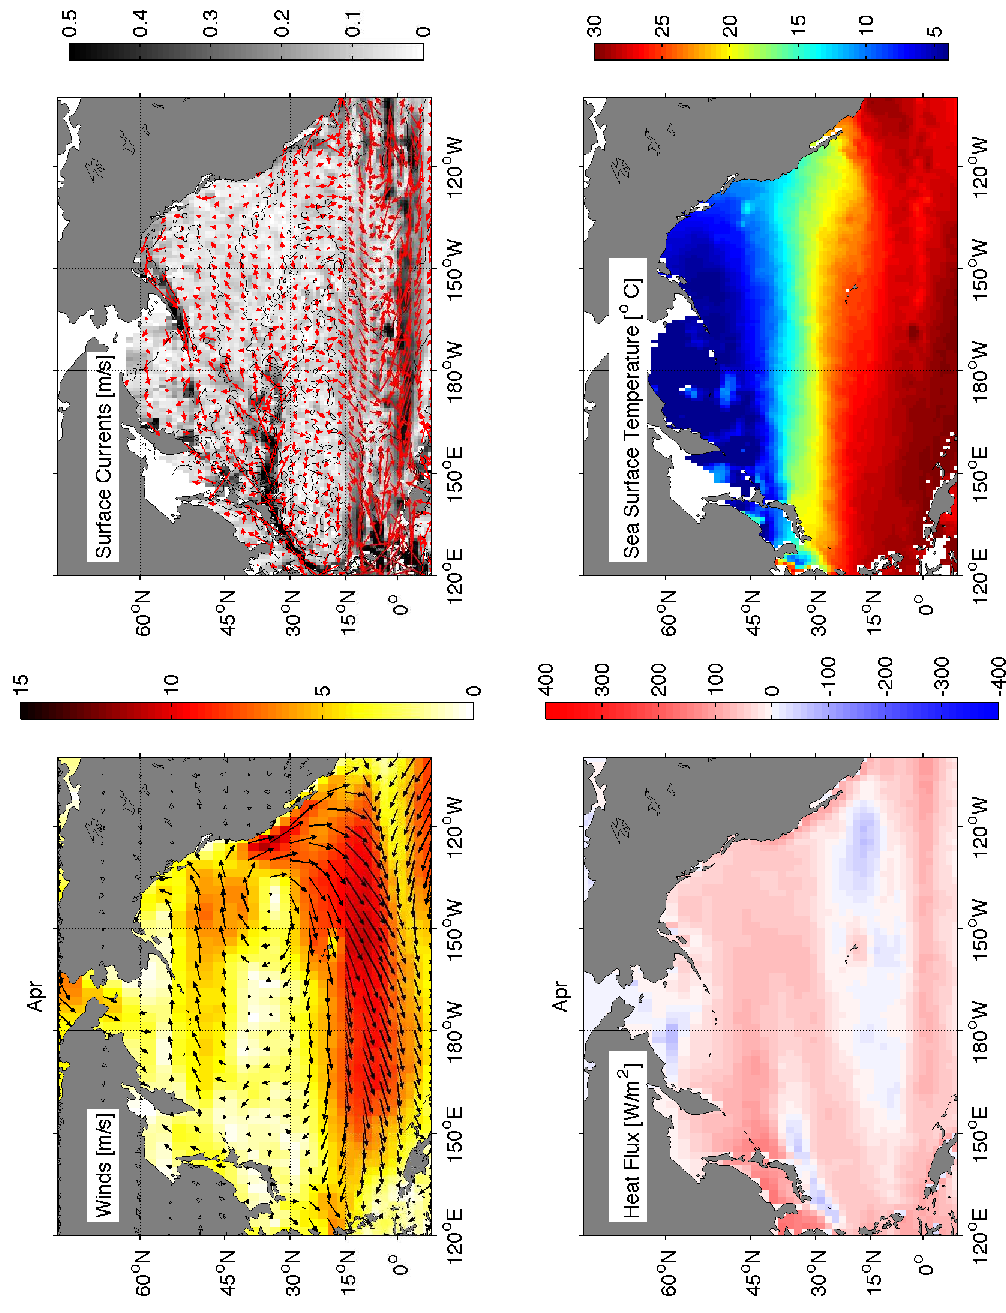
\includegraphics[angle=270]{figs/WindOverview/SurfaceCurrents04}
    \caption{}
    \label{fig:}  
  \end{center}
\end{figure}

\begin{figure}[hbt]
  \begin{center}
  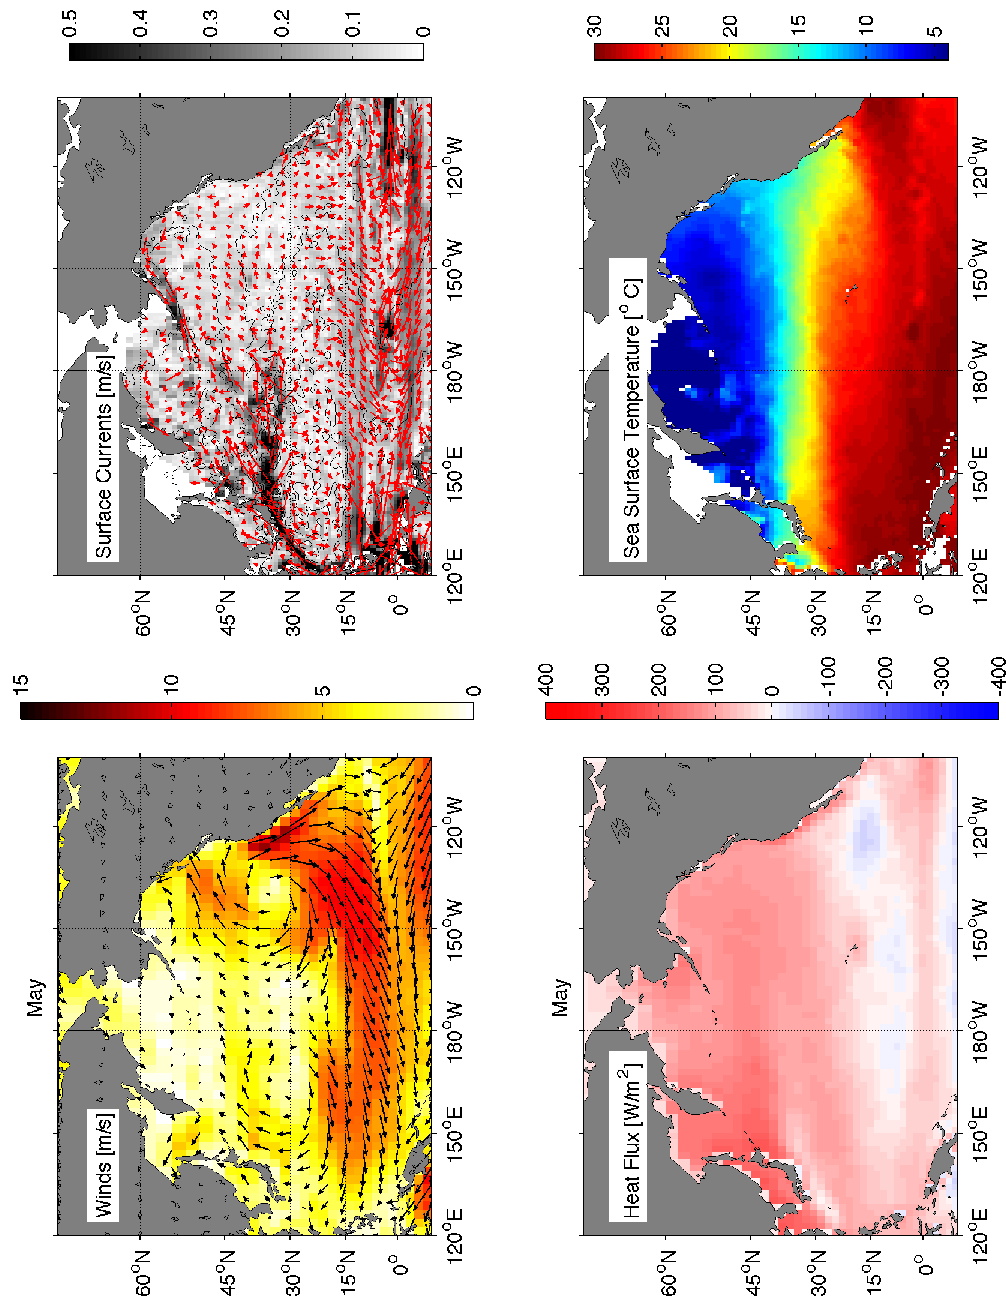
\includegraphics[angle=270]{figs/WindOverview/SurfaceCurrents05}
    \caption{}
    \label{fig:}  
  \end{center}
\end{figure}

\begin{figure}[hbt]
  \begin{center}
  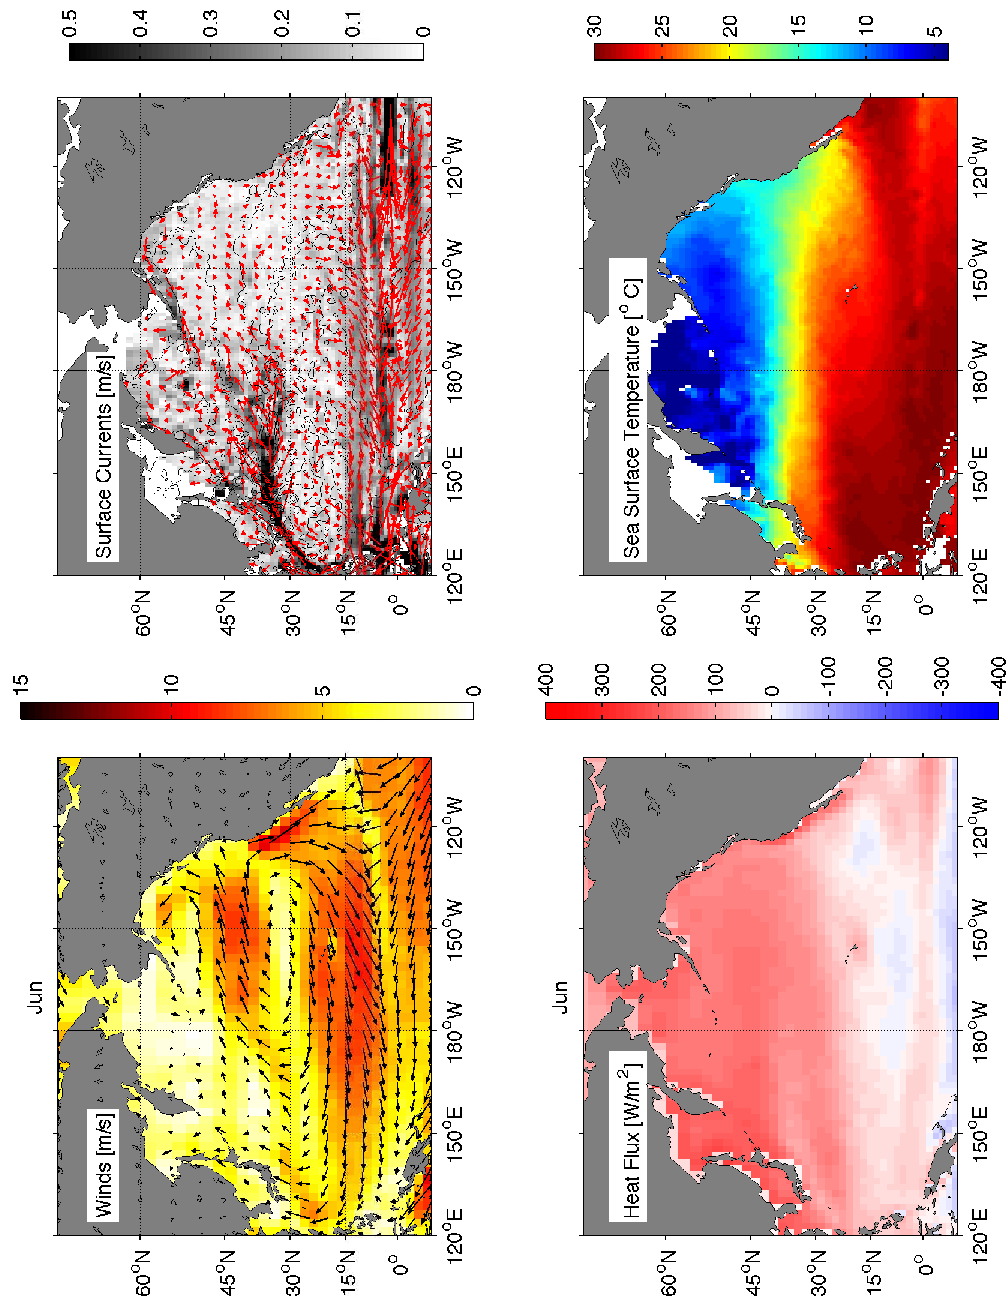
\includegraphics[angle=270]{figs/WindOverview/SurfaceCurrents06}
    \caption{}
    \label{fig:}  
  \end{center}
\end{figure}

\begin{figure}[hbt]
  \begin{center}
  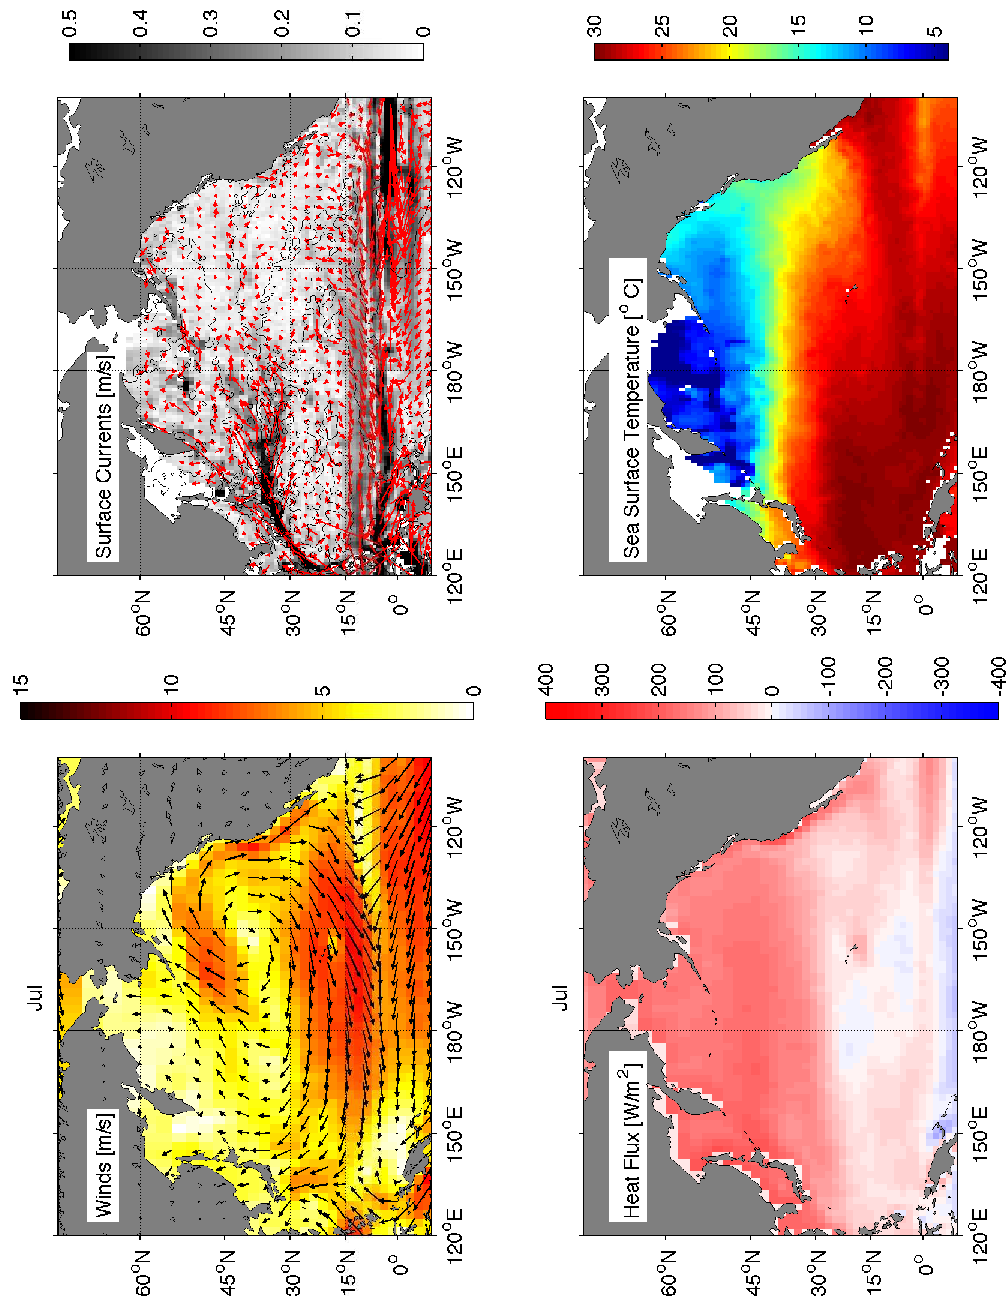
\includegraphics[angle=270]{figs/WindOverview/SurfaceCurrents07}
    \caption{}
    \label{fig:}  
  \end{center}
\end{figure}

\begin{figure}[hbt]
  \begin{center}
  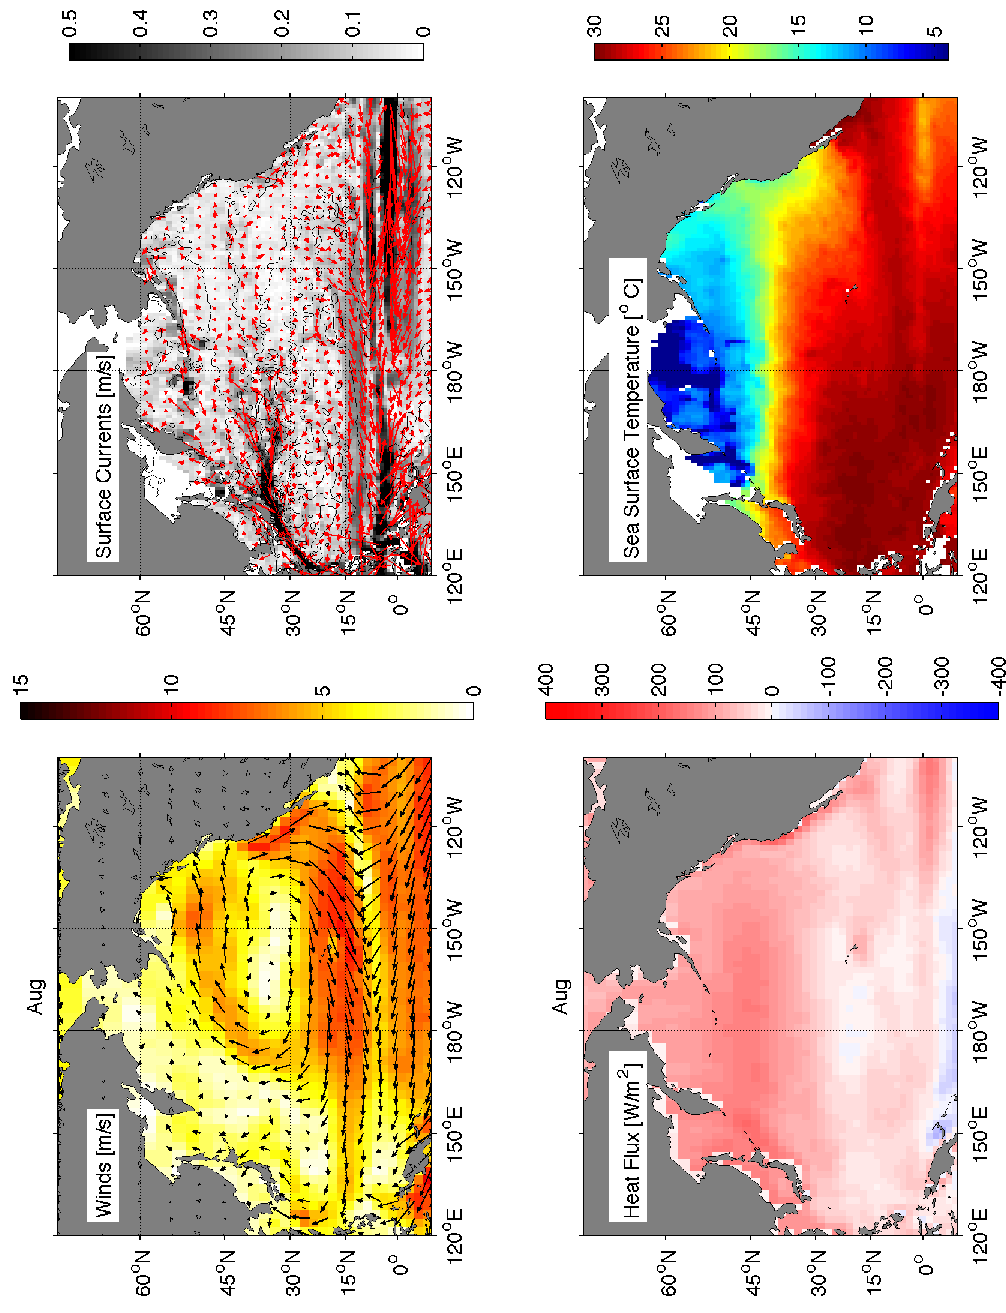
\includegraphics[angle=270]{figs/WindOverview/SurfaceCurrents08}
    \caption{}
    \label{fig:}  
  \end{center}
\end{figure}

\begin{figure}[hbt]
  \begin{center}
  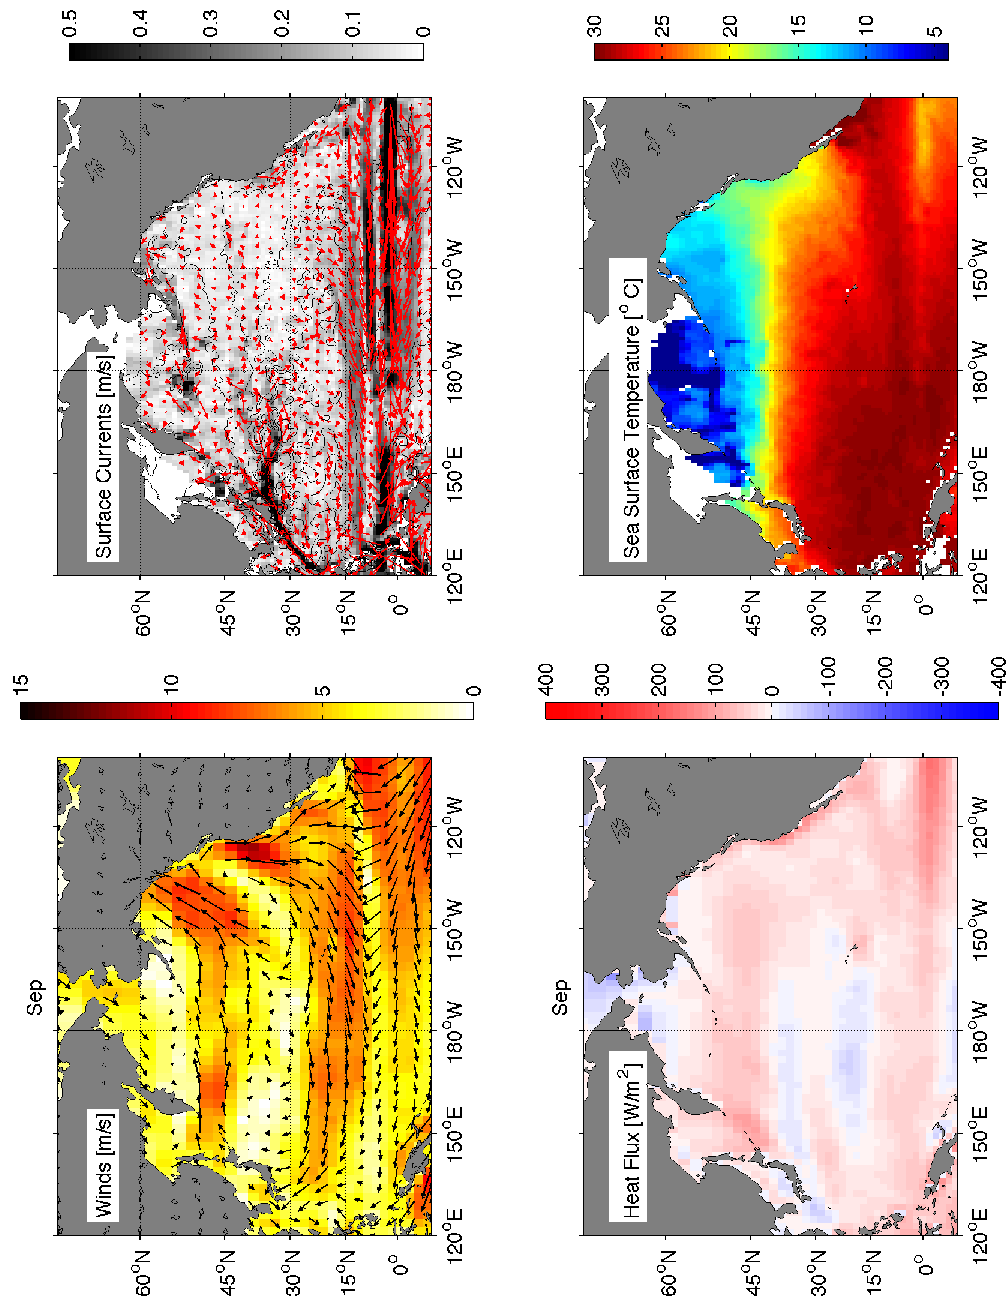
\includegraphics[angle=270]{figs/WindOverview/SurfaceCurrents09}
    \caption{}
    \label{fig:}  
  \end{center}
\end{figure}

\begin{figure}[hbt]
  \begin{center}
  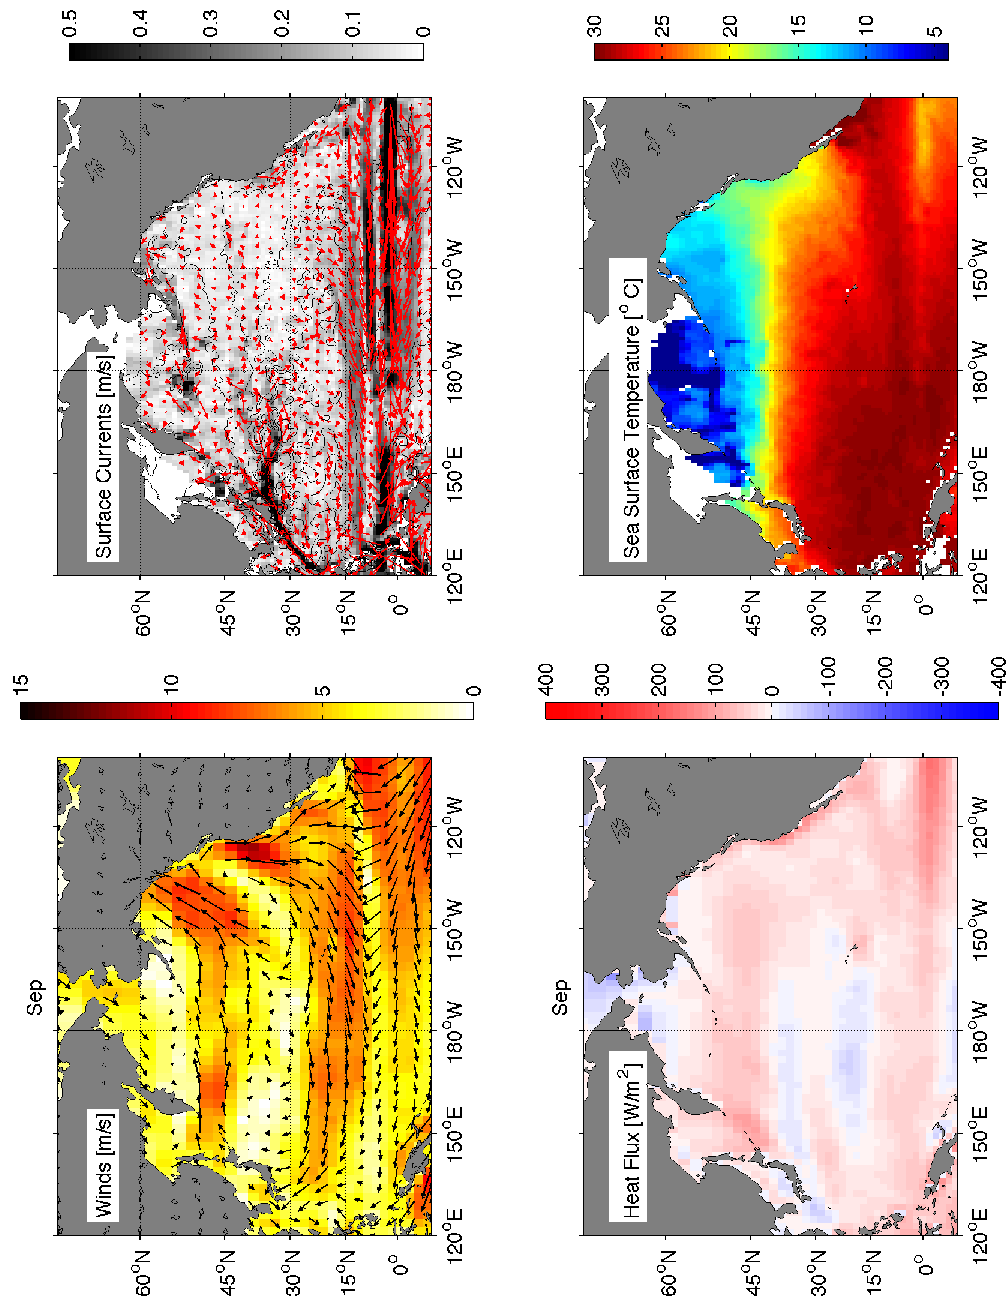
\includegraphics[angle=270]{figs/WindOverview/SurfaceCurrents09}
    \caption{}
    \label{fig:}  
  \end{center}
\end{figure}

\begin{figure}[hbt]
  \begin{center}
  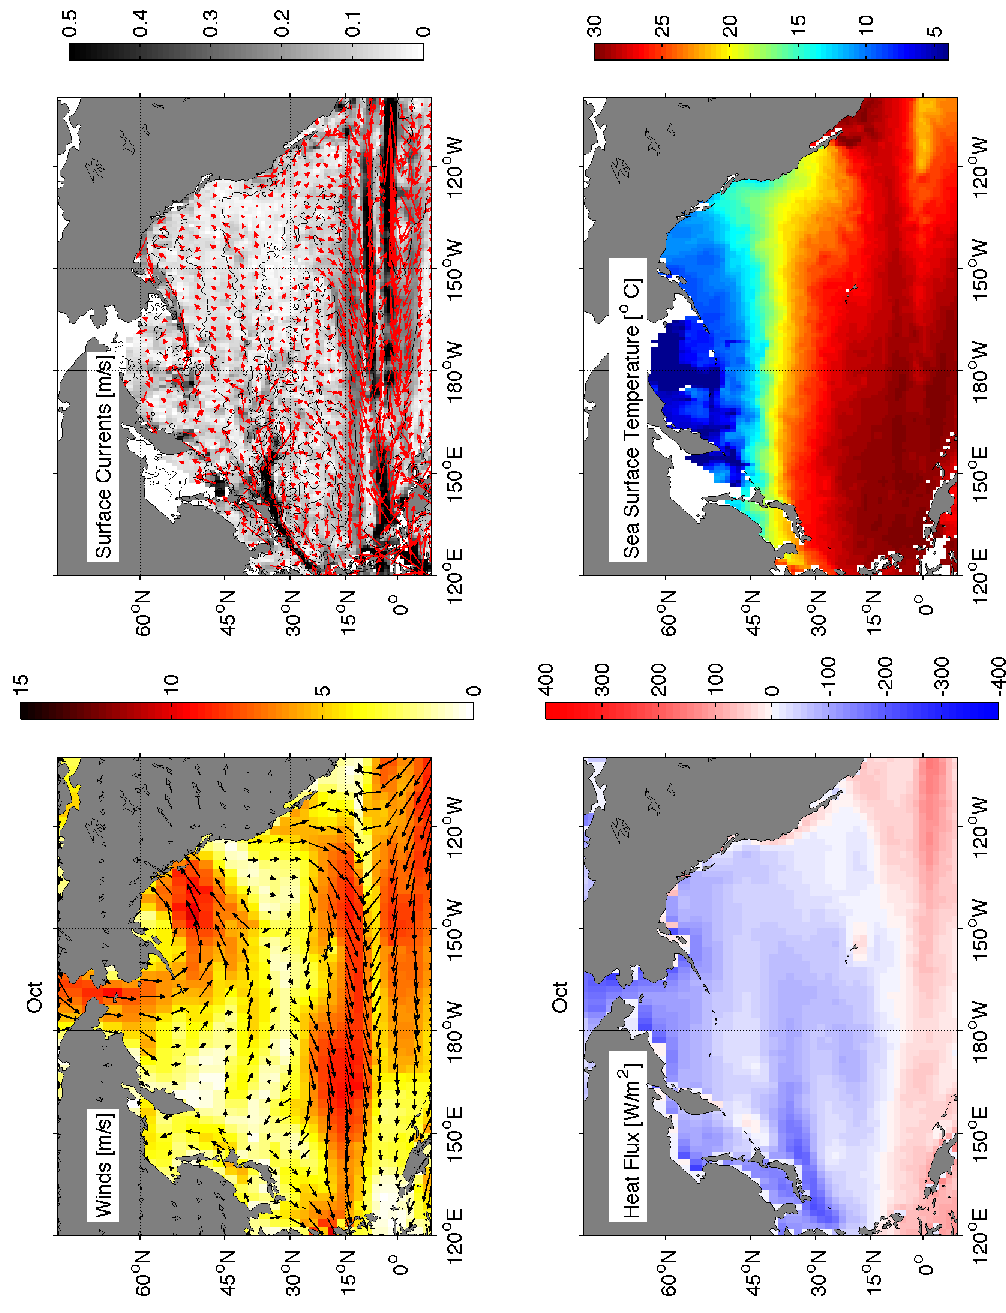
\includegraphics[angle=270]{figs/WindOverview/SurfaceCurrents10}
    \caption{}
    \label{fig:}  
  \end{center}
\end{figure}

\begin{figure}[hbt]
  \begin{center}
  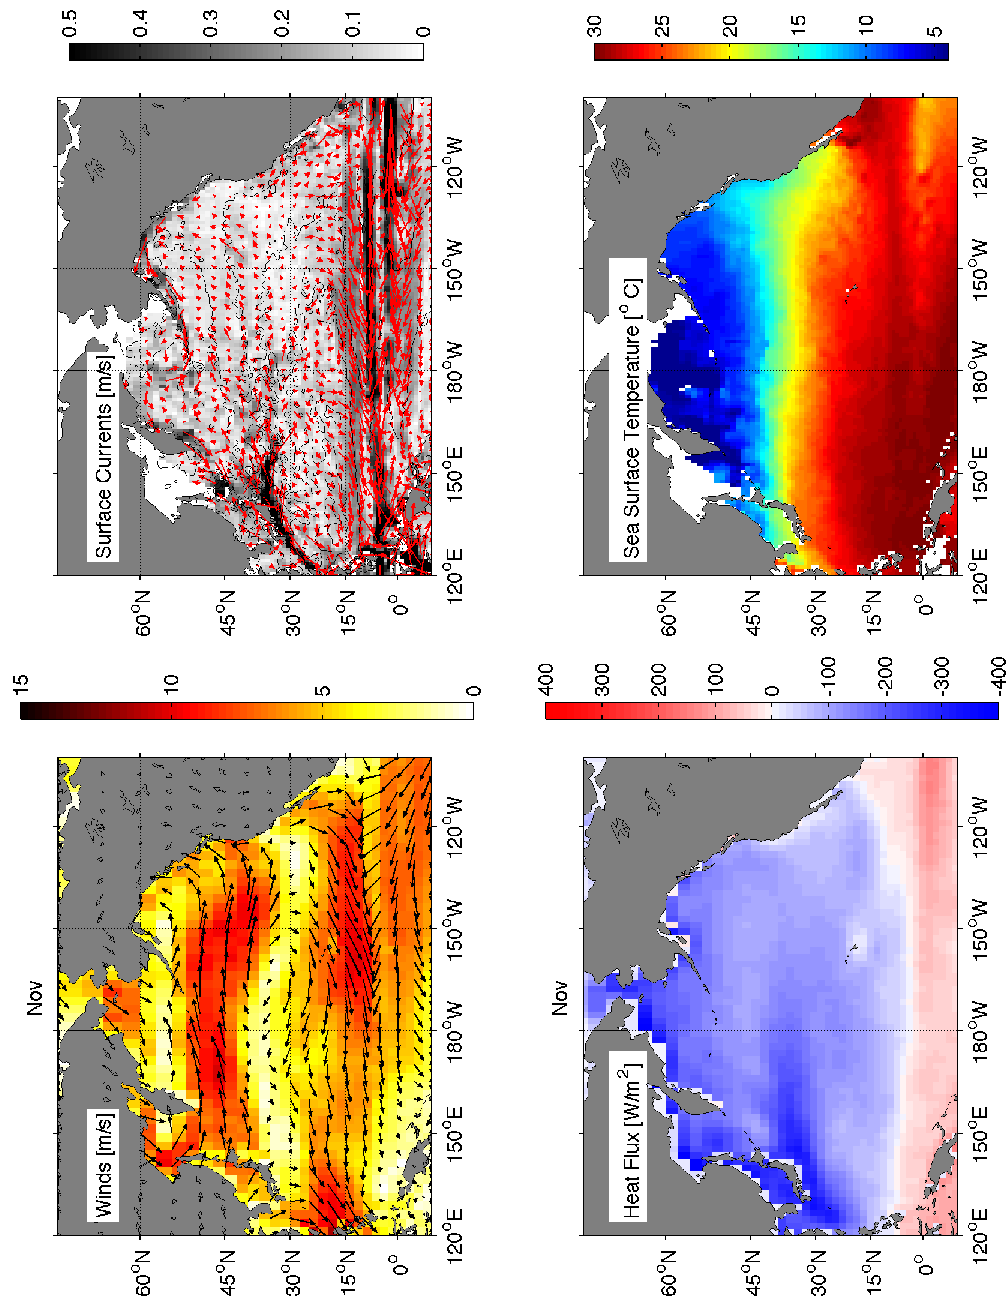
\includegraphics[angle=270]{figs/WindOverview/SurfaceCurrents11}
    \caption{}
    \label{fig:}  
  \end{center}
\end{figure}

\begin{figure}[hbt]
  \begin{center}
  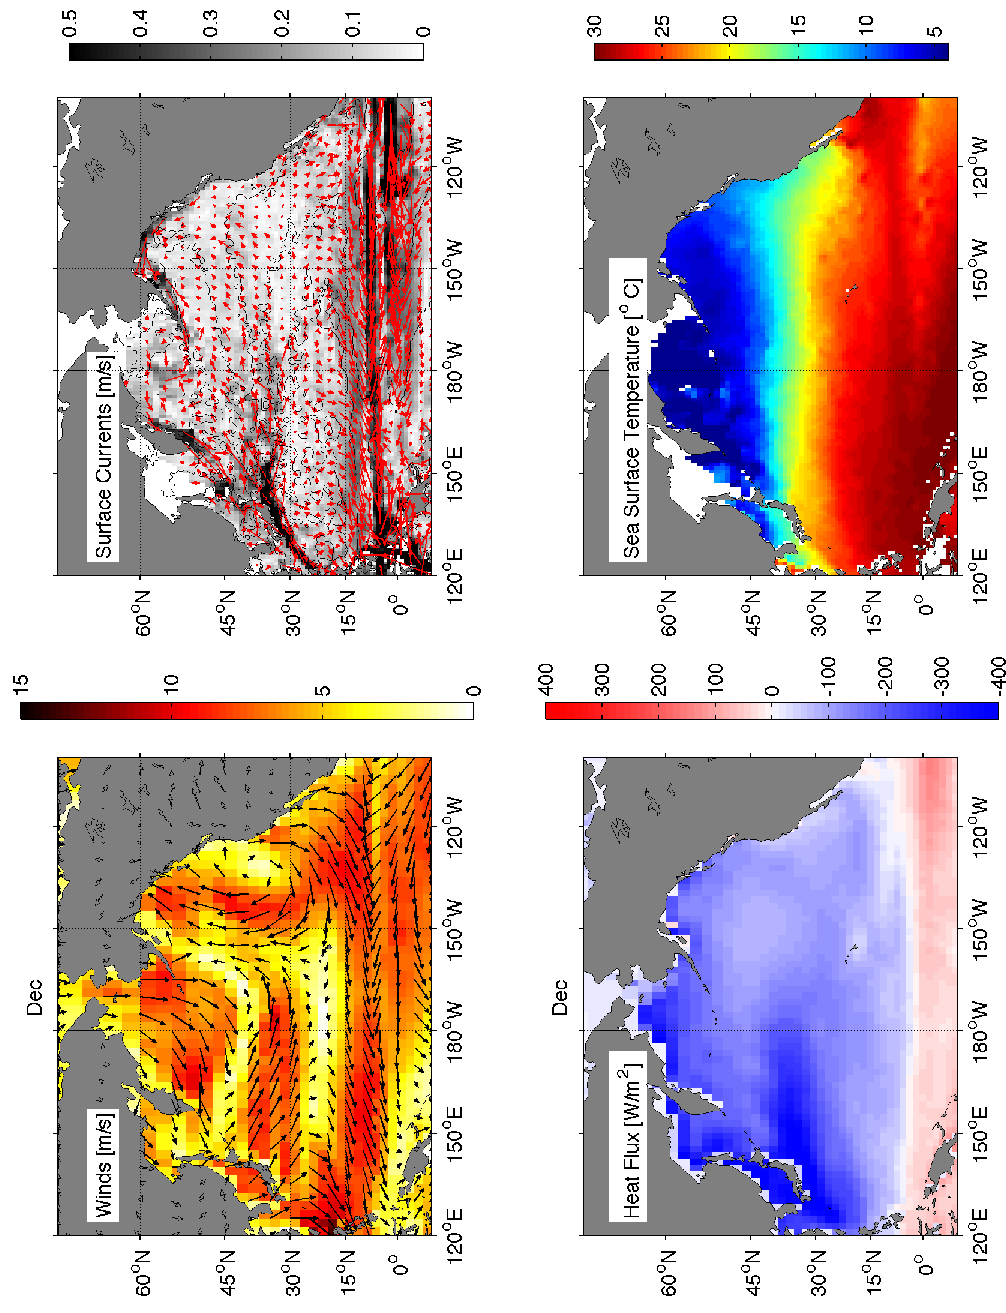
\includegraphics[angle=270]{figs/WindOverview/SurfaceCurrents12}
    \caption{}
    \label{fig:}  
  \end{center}
\end{figure}






%%% Local Variables:
%%% mode: latex
%%% TeX-master: t
%%% End:
